\section{Results}
\subsection{Transfer under a common decoding rule}
The two corpus pairs produce different outcomes under the same within-setting
comparison. FM improves VLR-to-ViCocktail transfer by 3.410 and 3.170 WER points
at seeds 17 and 29. It produces no clear LRS2-to-WildVSR improvement: the
common-decoder FC--FM difference is $-0.067$ points, with an interval that
includes zero. Figure~\ref{fig:gains} and Table~\ref{tab:comparisons} summarize
these contrasts. We first examine destination transfer and the corresponding
source assessment, then analyze error changes, training exposure and contextual
information.

\subsubsection{VLR to ViCocktail}

Table~\ref{tab:vi} presents the VLR-to-ViCocktail comparison. With the common
beam decoder, replacing half the full-clip presentations with fragments reduces
WER from 67.326 to 63.916 at seed 17 and from 67.233 to 64.062 at seed 29.
The gains of 3.410 and 3.170 percentage points therefore persist with the same
recognizer architecture, source-clip schedule, update count and decoding rule.
They measure the benefit of the training intervention under this continuation
budget, rather than a benefit from model-specific decoder selection.

\begin{table}[tbp]
\centering\small
\caption{Whole-utterance transfer from VLR to ViCocktail. WER (\%) is lower when better.}
\label{tab:vi}
\begin{tabular}{llrrl}
\toprule
Model & Seed & Primary & Common & Primary decoder \\
\midrule
Initial & -- & 70.057 & 70.034 & Greedy $b=-1$ \\
FC & 17 & 67.445 & 67.326 & Greedy $b=-1$ \\
FM & 17 & 61.882 & 63.916 & $\alpha=0.5$ \\
FM-ST & 17 & 62.002 & 63.919 & $\alpha=0.9$ \\
CP & 17 & 62.444 & 64.793 & $\alpha=0.5$ \\
FC & 29 & 66.983 & 67.233 & Greedy $b=-1$ \\
FM & 29 & 63.448 & 64.062 & Greedy $b=-1$ \\
Native ViCocktail & -- & 38.503 & 38.503 & $\alpha=0.1$ \\
\bottomrule
\end{tabular}
\par\smallskip\begin{minipage}{\linewidth}\footnotesize Primary decoders use 768 ViCocktail development clips. The common decoder has CTC weight 0.1 and beam size 40. FM-ST and CP have seed 17 only. The native reference uses different training data and preprocessing.
\end{minipage}
\end{table}


Development-selected decoding strengthens the seed-17 result: FC/FM obtain
67.445/61.882 WER, a 5.563-point gain. At seed 29, the corresponding values are
66.983/63.448, a 3.536-point gain. The interaction with decoding affects the
magnitude, but not the direction, of the Vietnamese result. FM also improves on
the uncontinued initializer, which obtains 70.057 primary and 70.034 common-decoder
WER. The native ViCocktail reference reaches 38.503 WER with different training
resources and preprocessing. FM thus improves cross-corpus continuation while
leaving a substantial gap to a system developed for the destination corpus.

Both seeds improve in all 20 original-video groups under either decoding regime.
The common-decoder source-bootstrap 95\% intervals are [2.892, 4.119] and
[2.683, 3.885] points (Table~\ref{tab:comparisons}; Figure~\ref{fig:gains}).
This consistency supports a gain within the studied corpus pair. The intervals
summarize variation across observed recording groups conditional on the fitted
models; they do not estimate variability across independently trained seeds.

\begin{table}[tbp]
\centering\small
\caption{Paired FC--FM improvements and 95\% bootstrap intervals (percentage points).}
\label{tab:comparisons}
\begin{tabular}{llrrr}
\toprule
Transfer & Seed & Regime & Gain & 95\% interval \\
\midrule
VI & 17 & Primary & 5.563 & [4.940, 6.351] \\
VI & 29 & Primary & 3.536 & [2.360, 4.768] \\
VI & 17 & Common & 3.410 & [2.892, 4.119] \\
VI & 29 & Common & 3.170 & [2.683, 3.885] \\
EN & 17 & Primary & 0.025 & [-0.371, 0.428] \\
EN & 17 & Common & -0.067 & [-0.338, 0.210] \\
\bottomrule
\end{tabular}
\par\smallskip\begin{minipage}{\linewidth}\footnotesize Positive values favor FM. Vietnamese intervals resample original-video groups; English intervals resample released clips. Intervals condition on the fitted models and decoders.
\end{minipage}
\end{table}


\begin{figure}[tbp]
 \centering
 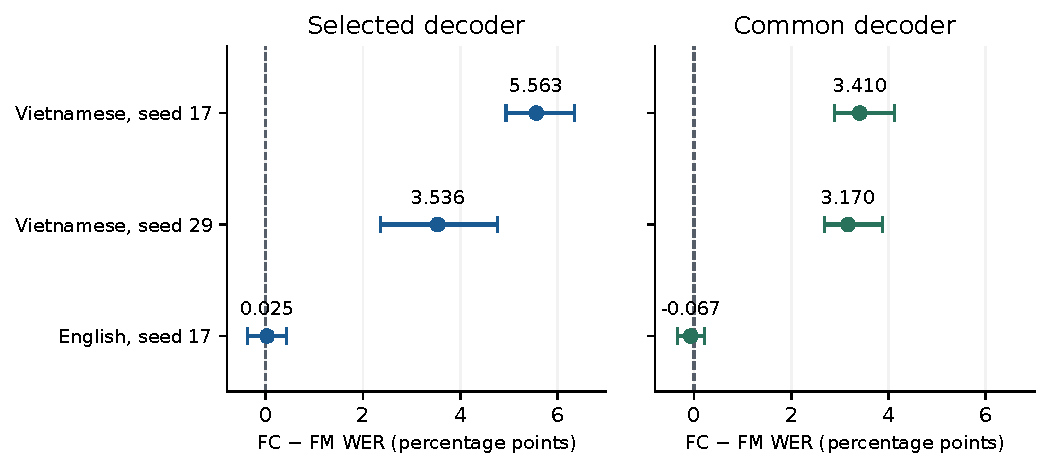
\includegraphics[width=\linewidth]{paired_gains.pdf}
 \caption{Paired FC--FM gains in whole-utterance WER. Positive values favor FM.
 Error bars are 95\% bootstrap intervals. Vietnamese intervals resample original
 videos; English intervals resample released clips. The English result provides
 a cross-setting check, without pooling the two languages.}
 \label{fig:gains}
\end{figure}

\subsubsection{LRS2 to WildVSR}

The English experiment checks the same recipe in a different continuation
setting. It does not reproduce the Vietnamese advantage (Table~\ref{tab:en}).
Primary FC/FM WER is 66.817/66.792: a 0.025-point gain with a conditional
clip-bootstrap interval of [$-0.371$, 0.428]. Under the common decoder, FM is
slightly worse, 66.884 versus 66.817, with an FC--FM interval of
[$-0.338$, 0.210]. The initializer obtains 66.164 primary and 67.092 common WER.
FM is therefore descriptively worse than the initializer under selected decoding,
but slightly better under common decoding; continuation is not uniformly helpful.

\begin{table}[tbp]
\centering\small
\caption{Whole-utterance transfer to WildVSR. WER (\%) on the same 2,854 assessment clips.}
\label{tab:en}
\begin{tabular}{llrrl}
\toprule
Model & Seed & Primary & Common & Primary decoder \\
\midrule
Initial & -- & 66.164 & 67.092 & $\alpha=0.5$ \\
FC & 17 & 66.817 & 66.817 & $\alpha=0.1$ \\
FM & 17 & 66.792 & 66.884 & $\alpha=0.5$ \\
FM-ST & 17 & 66.771 & 66.894 & $\alpha=0.5$ \\
CP & 17 & 66.749 & 66.794 & $\alpha=0.5$ \\
Full-pool FC & 17 & 67.438 & 67.438 & $\alpha=0.1$ \\
Large-data Auto-AVSR & -- & 36.010 & 36.010 & $\alpha=0.1$ \\
\bottomrule
\end{tabular}
\par\smallskip\begin{minipage}{\linewidth}\footnotesize Primary decoders use 1,082 LRS2 source-development clips. The common decoder has CTC weight 0.1 and beam size 40. All continuation variants use seed 17. Full-pool FC changes the training population; the large-data reference uses different pretraining resources.
\end{minipage}
\end{table}


The training regimes differ materially. English fragment eligibility retains
7,291 of 45,838 prepared clips (15.91\%), increasing mean training duration from
2.183 to 4.404 seconds. Each eligible clip is presented six or seven times,
whereas each selected Vietnamese clip appears once. Using the complete English
pool in the equal-step F0 control gives 67.438 WER, worse than matched-pool FC
by 0.620 points (95\% interval [0.298, 0.950]). This alternative does not recover
the gain; it changes content, duration and repetition together, and cannot show
that additional data is intrinsically harmful.

The assessment durations are more similar: Vietnamese mean/median length is
145.74/129 frames, versus 151.31/139 in English. English's largest length stratum
is nearly tied and the stratum above 200 frames is slightly worse with FM.
The contrast therefore cannot be explained simply by shorter English test clips.
The larger-data English reference reaches 36.010 WER, emphasizing the remaining
gap to stronger training resources. Taken together, the English results bound
the portability of FM and motivate studying exposure and supervision conditions,
rather than attributing the difference to language alone.

\subsection{Does the gain require fixed-time boundary supervision?}
\label{sec:cropresults}
The matched augmentation follow-up directly compares fixed-time fragments with
conventional whole-word views (Section~\ref{sec:matchedcrop}). Table~\ref{tab:crop}
shows the four matched states under the common decoder. We first compare the
three crop-control states. Fixed-time mixing
reduces WER from 67.369 to 63.846, a 3.523-point gain with a conditional
95\% group-bootstrap interval of [2.985, 4.179]. Whole-word mixing reaches
63.388 WER, improving over full-only by 3.981 points \mbox{[3.420, 4.731]}.

\begin{table}[tbp]
\centering\small
\setlength{\tabcolsep}{4pt}
\caption{Source and destination performance of the matched continuation recipes
at seed 17. The same fitted states use a common decoder on 11,307 VLR and
1,167 ViCocktail clips. Training frame and native-token counts are in millions.}
\label{tab:crop}
\begin{tabular}{lrrrr}
\toprule
Training views & VLR WER (\%) & ViCocktail WER (\%) & Frames & Tokens\\
\midrule
Full-only & 38.029 & 67.369 & 7.307 & 1.145\\
Fixed-time mixed & 38.580 & 63.846 & 4.888 & 0.798\\
Whole-word mixed & 38.606 & 63.388 & 5.013 & 0.784\\
Whole-word short-only & 44.844 & 70.715 & 2.719 & 0.422\\
\bottomrule
\end{tabular}
\par\smallskip\begin{minipage}{\linewidth}\footnotesize
Each arm uses 48,000 source presentations and 6,000 updates. Both mixed arms
share 317 full-clip fallbacks; short-only uses 598 fallbacks (1.25\%).
These fitted states are distinct from the original FC/FM comparison.
Frame and token exposures are not equal.
\end{minipage}
\end{table}


Whole-word mixing is better than fixed-time mixing by 0.459 points
[0.268, 0.674]. Its 138 fewer errors comprise 106 fewer deletions and 78 fewer
insertions, offset by 46 additional substitutions. The transfer benefit thus
persists with conventional word-aligned views, and the tested fixed-time rule
does not provide an additional advantage over the tested whole-word alternative
under this protocol. This supports mixed short supervision
as a useful continuation choice here without requiring incomplete boundary
evidence as its explanation.

The same three fitted states also expose the source cost of these transfer
gains. On all 11,307 VLR test clips, WER is 38.029 for full-only, 38.580 for
fixed-time and 38.606 for whole-word continuation. Relative to full-only,
the source costs are 0.551 points [0.439, 0.664] for fixed-time and
0.577 points [0.448, 0.705] for whole-word mixing. Both arise primarily from
more deletions, despite fewer substitutions. Whole-word source WER exceeds
fixed-time WER by 0.026 points, with an interval of [$-0.043$, 0.091].
This comparison does not resolve a source-performance difference between the
two crop rules or establish their equivalence. Whole-word mixing delivers the
larger measured destination gain; neither mixed recipe improves uniformly
over full-only continuation across source and destination.

The three crop-control arms receive the same source presentations and updates. Whole-word
mixing nevertheless processes 2.55\% more frames and 1.70\% fewer target tokens
than fixed-time mixing. The comparison therefore evaluates two practical crop
recipes rather than isolating a single boundary variable. It is a one-seed
follow-up on the previously used assessment corpus, with shared fallback
positions. The original FM source/destination profile below belongs to different
fitted states; Table~\ref{tab:crop} reports the new controls' own source assessment.

\subsection{Does the gain persist without scheduled full-clip supervision?}
\label{sec:shortonlyresults}
The short-only state obtains 70.715\% ViCocktail WER and 44.844\% VLR WER
(Table~\ref{tab:crop}). The predeclared whole-word mixed--short-only differences
are $-7.328$ destination points [${-8.864}$, ${-5.488}$] and $-6.238$ source
points [${-6.592}$, ${-5.887}$], favoring mixing in both populations.
Short-only is also worse than full-only continuation by 3.347 destination
points and 6.815 source points (Table~\ref{tab:shortonly}).

\begin{table}[tbp]
\centering\small
\caption{Predeclared comparisons with whole-word short-only continuation.
Differences are reference minus short-only WER in percentage points;
positive values favor short-only. Mixed denotes whole-word mixing.}
\label{tab:shortonly}
\begin{tabular}{llrr}
\toprule
Population & Contrast & Difference & 95\% interval\\
\midrule
VLR & Mixed--short-only & -6.238 & [-6.592, -5.887]\\
VLR & Full--short-only & -6.815 & [-7.207, -6.440]\\
ViCocktail & Mixed--short-only & -7.328 & [-8.864, -5.488]\\
ViCocktail & Full--short-only & -3.347 & [-4.773, -1.341]\\
\bottomrule
\end{tabular}
\par\smallskip\begin{minipage}{\linewidth}\footnotesize
Pointwise intervals use 10,000 paired bootstrap resamples of 61 archived
VLR source groups or 20 ViCocktail recording groups, conditional on the fitted
states. Whole-word mixed versus short-only is the primary contrast;
full-only versus short-only is the reference contrast.
\end{minipage}
\end{table}


The loss is dominated by deletions. Relative to whole-word mixing, short-only
adds 5,735 deletions on ViCocktail; 3,098 fewer substitutions and 432 fewer
insertions leave 2,205 additional errors. On VLR, 33,541 additional deletions
outweigh 15,373 fewer substitutions and 4,072 fewer insertions, adding 14,096
errors. This error balance is consistent with poorer complete-transcript coverage,
but does not identify its internal cause.

Retaining scheduled full-utterance presentations therefore improves the tested
whole-word recipe at the same update budget. The benefit of mixing over full-only
continuation cannot be extended to a nearly all-short schedule: the latter uses
47,402 short views and 598 full fallbacks, and performs worse than both controls.
Frame and target-token exposure also decrease, so this comparison does not
isolate context length from objective exposure or establish an optimal mixing ratio.

\subsection{Does the transfer gain persist under token-normalized loss?}
\label{sec:lossresults}
The paired reduction control tests whether the fixed-time gain depends on
retaining the native unnormalized components. Table~\ref{tab:reduction} reports
the complete four-state comparison. With token-normalized loss, full-only and
fixed-time mixing obtain 67.223 and 63.763 WER. The gain is 3.460 points,
with a conditional 95\% recording-group interval of [2.756, 4.423].

\begin{table}[tbp]
\centering\small
\caption{Loss-reduction control on the complete ViCocktail assessment at seed 17.
All four fitted states use the common decoder. Gain is full-only minus fixed-time WER.}
\label{tab:reduction}
\begin{tabular}{lrrr}
\toprule
Loss reduction & Full-only WER & Fixed-time WER & Gain (pp)\\
\midrule
Native & 67.369 & 63.846 & 3.523\\
Token-normalized & 67.223 & 63.763 & 3.460\\
\bottomrule
\end{tabular}
\end{table}


The normalized-minus-native change in the gain is $-0.063$ points, with a
paired interval of [$-0.366$, 0.386]. Thus the transfer advantage remains under
the tested component-wise normalization. The interval does not establish exact
equivalence between reductions, but the result does not support an explanation
in which the gain disappears after dividing by target length. This one-seed
control strengthens the short-view finding under a second objective reduction;
it does not identify a unique optimization mechanism or predict how normalized
whole-word mixing would behave.

\subsection{Source and destination performance at the same fitted states}
\label{sec:source}
For the original continuation comparison, we assess the initializer, FC and FM
on the complete prepared source test sets:
11,307 VLR clips and 1,243 LRS2 clips. This retrospective follow-up uses the
same seed-17 checkpoints and readouts as the destination comparison, without
source-test decoder tuning. Table~\ref{tab:source} and Figure~\ref{fig:source}
show the resulting source/destination profiles.

\begin{table}[tbp]
\centering\small
\caption{Source and destination WER (\%) at the same fitted states and
common decoder. Source populations are 1,243 LRS2 clips (6,660 words)
and 11,307 VLR clips (225,960 whitespace units). Destination populations
are 2,854 WildVSR and 1,167 ViCocktail clips. Continuation results use seed 17;
each corpus is scored separately. Lower WER is better.}
\label{tab:source}
\begin{tabular}{lrrrr}
\toprule
& \multicolumn{2}{c}{English} & \multicolumn{2}{c}{Vietnamese}\\
\cmidrule(lr){2-3}\cmidrule(lr){4-5}
State & LRS2 & WildVSR & VLR & ViCocktail\\
\midrule
Initializer & 56.577 & 67.092 & 39.830 & 70.034\\
FC & 50.976 & 66.817 & 38.016 & 67.326\\
FM & 52.432 & 66.884 & 38.604 & 63.916\\
\bottomrule
\end{tabular}
\end{table}


On VLR, common-decoder WER is 39.830 for the initializer, 38.016 for FC and
38.604 for FM. The paired FC--FM difference is $-0.588$ points, with a
95\% source-group bootstrap interval of [$-0.709$, $-0.474$]. FM therefore
trades a modest source disadvantage relative to FC for its 3.410-point
ViCocktail improvement at this seed. It adds 1,329 source errors: 3,641
additional deletions outweigh 2,163 fewer substitutions and 149 fewer
insertions. Both continuations still improve on the initializer.

On LRS2, common-decoder WER is 56.577, 50.976 and 52.432 for the initializer,
FC and FM. FM produces 97 more errors than FC: 32 substitutions, 26 deletions
and 39 insertions across 6,660 reference words. The FC--FM difference is
$-1.456$ points, with an interval of [$-2.375$, $-0.584$]. Unlike the
Vietnamese profile, this source disadvantage has no demonstrated destination
benefit on WildVSR. It is a disadvantage relative to FC, not forgetting
relative to the initializer; the experiment does not measure the English
initializer's upstream LRS3 performance.

Decoder selection changes the Vietnamese source ranking. Applying the frozen
ViCocktail-development choices to VLR gives FC/FM WERs of 43.371/38.939 and
an FC--FM difference of 4.432 points [4.199, 4.658]. FC uses greedy CTC with
blank bias $-1$, whereas FM uses hybrid beam decoding with CTC weight 0.5.
These are destination-calibrated readouts, not source-optimal decoders, and
their contrast combines changes in the fitted model and decoding. The common
decoder exposes the smaller source cost described above. The English source
ranking is unchanged by its development-selected readouts: FC/FM WER is
50.976/52.883, a difference of $-1.907$ points [$-2.986$, $-0.831$].

\begin{figure}[tbp]
 \centering
 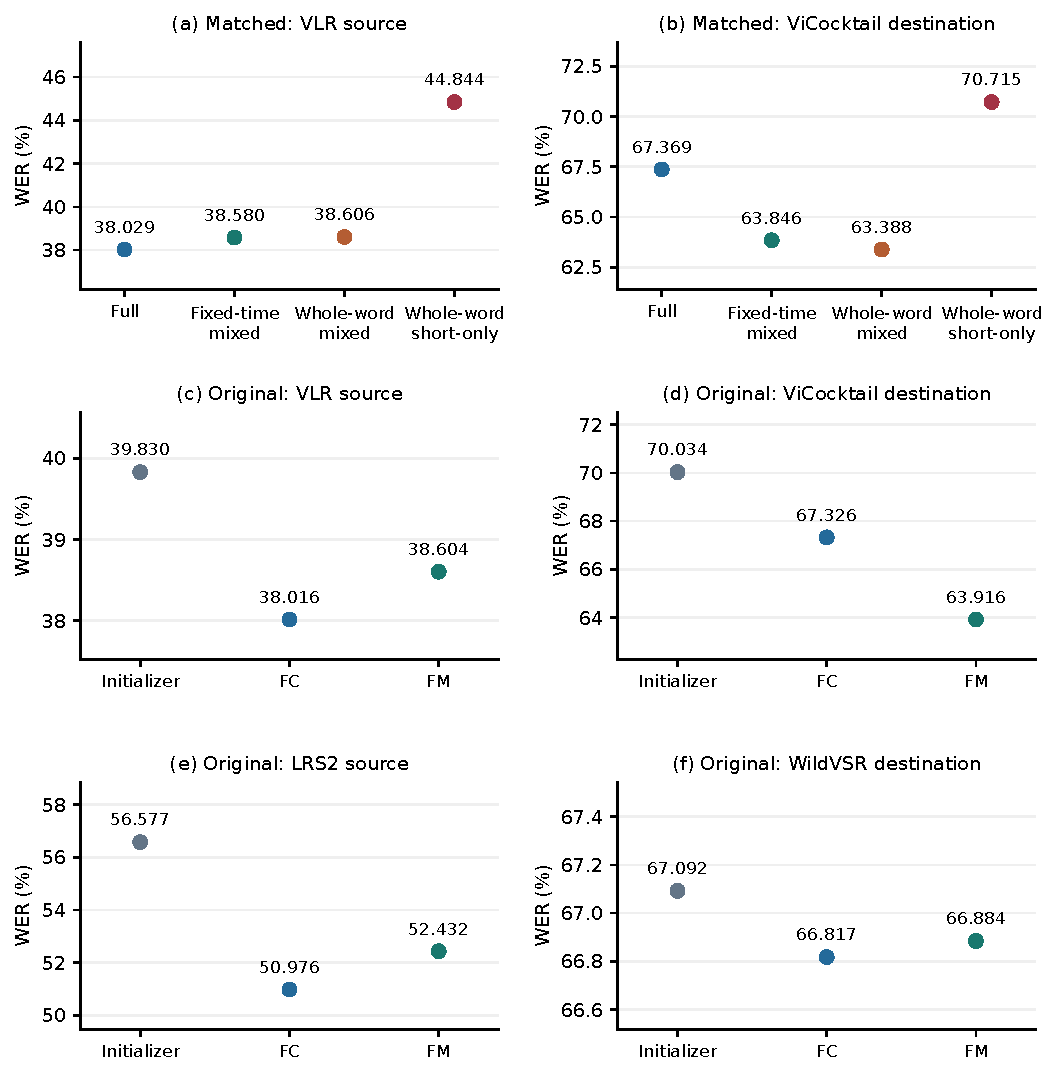
\includegraphics[width=\linewidth]{source_destination_profile.pdf}
 \caption{Source/destination WER at the same fitted seed-17 states under common
 decoding. (a,b) The matched full-only, fixed-time mixed, whole-word mixed and
 short-only states. (c,d) The original Vietnamese initializer/FC/FM comparison.
 (e,f) The original English comparison. Original and matched FC/FM states are
 distinct. Each panel has a separately labelled vertical scale; WERs are not
 averaged across corpora.}
 \label{fig:source}
\end{figure}

The source follow-up separates a transfer benefit from uniform improvement
across corpora. It also shows why source retention must be reported with its
readout: a ranking obtained with destination-calibrated decoders need not
match the ranking under shared decoding. Neither profile identifies the
learning mechanism responsible for the difference between continuation settings.

\subsection{Error changes and utterance length}
Under the common decoder, Vietnamese FM removes 1,026 errors at seed 17:
34 substitutions, 492 deletions and 500 insertions. At seed 29, it removes
954 errors: 35 substitutions, 371 deletions and 548 insertions
(Figure~\ref{fig:errors}). Most of the gain therefore comes from producing a
more accurate number of transcript units, rather than substituting fewer units.
The counts are consistent with a change in omission--insertion behavior; they
do not identify whether the cause lies in visual representations, attention
or confidence calibration.

\begin{figure}[tbp]
 \centering
 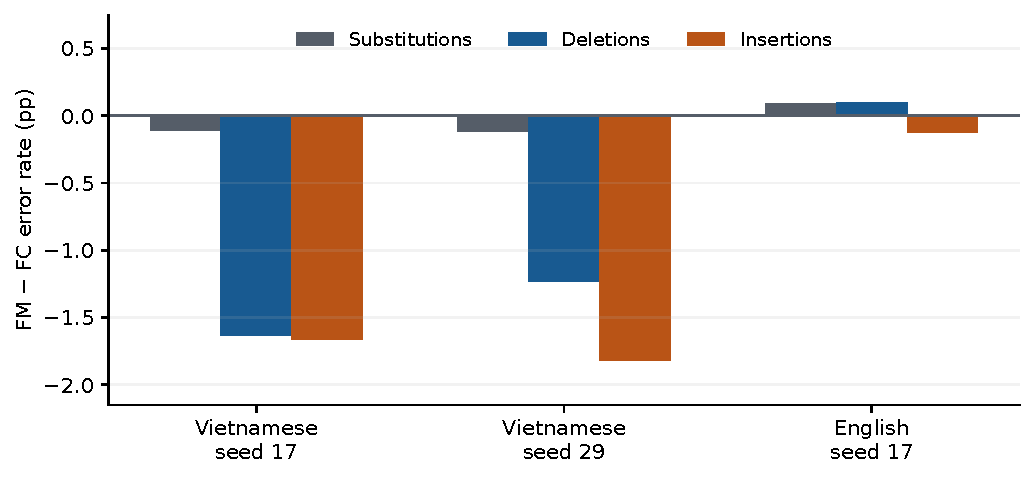
\includegraphics[width=\linewidth]{edit_changes.pdf}
 \caption{Common-decoder changes in substitution, deletion and insertion rates,
 computed as $100(\text{FM count}-\text{FC count})/N$. Negative values indicate
 fewer errors. Each setting uses its own complete assessment reference count.}
 \label{fig:errors}
\end{figure}

A post-hoc length analysis shows that the Vietnamese gain extends beyond short
utterances. The largest stratum, 101--200 prepared frames, contains 772 clips and
17,820 reference units. FM removes 398 and 349 errors at seeds 17 and 29,
respectively, reducing WER by 2.233 and 1.958 points. Clips above 200 frames also
improve, by 3.814 and 3.275 points. The 11 shortest clips contain only 57 reference
units and account for 58 and 63 errors removed; their extreme percentage-point
changes do not characterize the aggregate result. These descriptive strata were
formed after inspecting the aggregate outcomes.

\subsection{Training exposure and the role of context}
\label{sec:exposure}
FM changes the length of both the visual input and its supervision.
Table~\ref{tab:exposure} quantifies this change at the common final update.
Vietnamese FM uses approximately 66.4\% of FC's input frames and 69.1\% of its
target tokens in both seeds. Equal numbers of updates and presentations therefore
do not imply equal information exposure. These counts do not measure FLOPs,
runtime or gradient scale.

\begin{table}[tbp]
\centering\small
\caption{Training exposure at 6,000 updates. Every run has 48,000 presentations;
frame and native-token counts are shown in millions.}
\label{tab:exposure}
\begin{tabular}{llrrrr}
\toprule
Setting & Seed & FC frames & FM frames & FC tokens & FM tokens\\
\midrule
Vietnamese & 17 & 7.307 & 4.851 & 1.145 & 0.791\\
Vietnamese & 29 & 7.293 & 4.842 & 1.144 & 0.790\\
English & 17 & 5.284 & 3.843 & 0.831 & 0.629\\
\bottomrule
\end{tabular}
\end{table}

The two context controls retain FM's fragment targets. CP supplies neighboring
pixels, adding 768,000 encoder input frames across 24,000 fragment presentations.
FM-ST instead supplies a full-view predictive distribution through 24,000
additional teacher passes. At seed 17, total encoder input is 76.90\% of FC for
Vietnamese CP and 116.42\% for FM-ST (Figure~\ref{fig:contextbudget}). Teacher
passes do not backpropagate, so the ratios are exposure comparisons rather than
compute-matched budgets.

\begin{figure}[tbp]
 \centering
 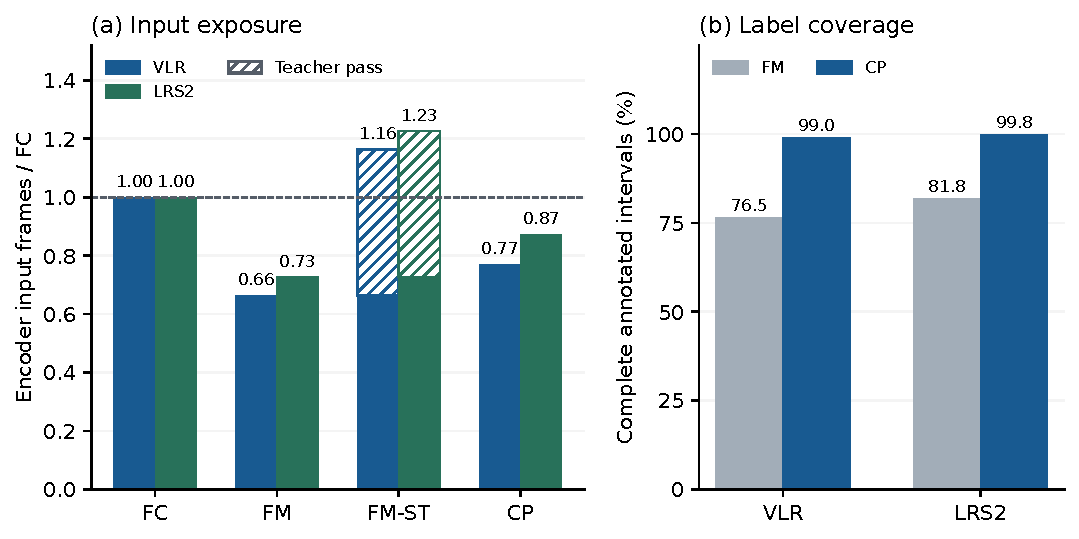
\includegraphics[width=\linewidth]{training_context_budget.pdf}
 \caption{Training-design measurements at seed 17. (a) Encoder input frames
 relative to FC, including the no-gradient teacher pass in FM-ST. (b) Selected
 positive-duration annotation intervals fully contained in the encoder input.
 Coverage uses all 24,000 fragment presentations per corpus and automatic
 timestamps; zero-duration entries are excluded.}
 \label{fig:contextbudget}
\end{figure}

Added context also restores visual evidence for labels touching a crop boundary.
The fraction of selected positive-duration annotation intervals fully contained
in the input rises from 76.49\% to 99.02\% in VLR, and from 81.79\% to 99.77\%
in LRS2. A one-frame tolerance preserves this contrast. The 2,378 zero-duration
VLR entries are excluded from coverage calculations but remain in training.
Thus, CP changes neighboring information and boundary-label coverage together;
it is not a pure intervention on context independent of label completeness.
Automatic timings describe annotation coverage, not verified visual articulation.

Neither control strengthens the main Vietnamese result. FM-ST reaches 62.002
primary and 63.919 common-decoder WER, compared with FM's 61.882 and 63.916.
The common-decoder difference is one error across 30,091 reference units; both
paired intervals include zero. The tested self-teaching loss therefore adds no
clear benefit at its specified temperature and weight.

CP reaches 62.444 primary and 64.793 common-decoder WER. It remains better than
FC by 5.001 and 2.532 points, but FM outperforms CP by 0.562 points under the
primary decoder (95\% interval [0.340, 0.826]) and 0.877 points under the common
decoder ([0.348, 1.422]). FM and CP select the same primary decoder.
Restoring most boundary-label coverage preserves a substantial benefit over FC,
while failing to improve FM. This supports further investigation of shorter
supervision; it does not establish that missing context causes the gain.

\begin{figure}[tbp]
 \centering
 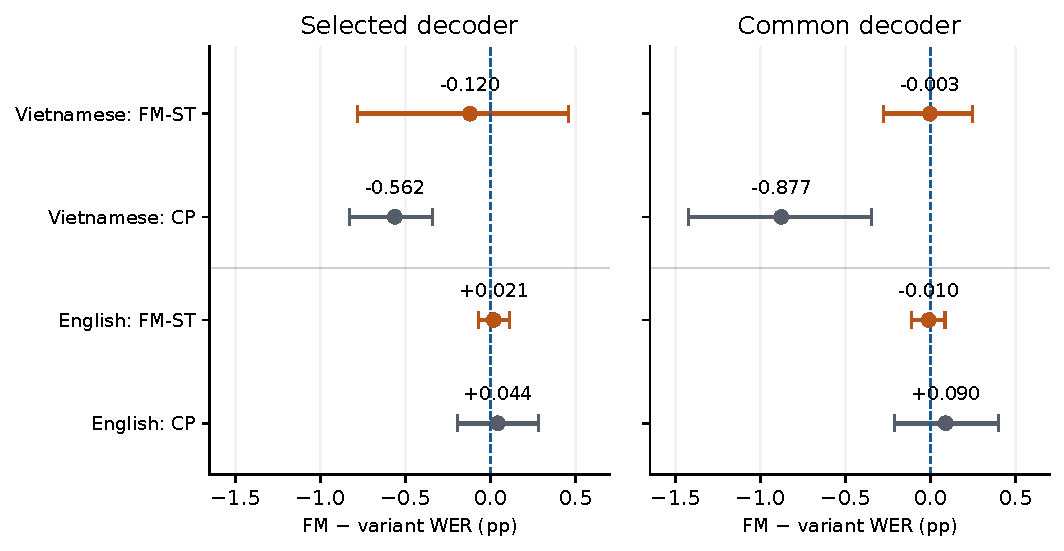
\includegraphics[width=\linewidth]{mechanism_gains.pdf}
 \caption{Paired effects of full-view self-teaching (FM-ST) and context
 preservation (CP) relative to FM at seed 17. Positive values favor the variant.
 Error bars are pointwise 95\% bootstrap intervals, conditional on fitted models
 and decoders, without multiple-comparison adjustment. Vietnamese resampling
 uses original-video groups; English resampling uses released clips.}
 \label{fig:mechanisms}
\end{figure}

CP's Vietnamese error balance differs from FM: 325 fewer substitutions and six
fewer insertions are offset by 595 additional deletions, producing 264 more
errors overall. This post-hoc decomposition shows why restoring visual coverage
or reducing one edit type need not improve complete-transcript WER.


In the English setting, FM-ST and CP remain near FM: their primary WERs are 66.771 and 66.749,
respectively, and all English FM--variant intervals include zero. Under the
common decoder, CP removes 621 substitutions and 461 insertions relative to FM
but adds 1,039 deletions, leaving only 43 fewer errors (0.090 points).
Likewise, common-decoder FM removes 59 insertions relative to FC but adds
44 substitutions and 47 deletions. The Vietnamese improvement in both insertion
and deletion counts does not carry over to this English setting.


